\section{Analysis}\label{sec:results_web_ping} % TODO Better section name?
\subsection{Initial Site Ping Analysis}
For initial analysis we we used D3.js to allow for live results to be displayed on the website. This analysis was done by aggregating the data on the server side by state and by city. They were automatically updated with every new data point. to both allow us to perform some preliminary analysis and allow users to see how there respective state is doing.

\begin{figure}
    \centering
    \includegraphics[width=\textwidth]{images/siteping/Sitping_Rankings.png}
    \caption{The rankings displayed on the site.}
    \label{fig:siteping_rankings}
\end{figure}

Initially, we also displayed the data live, both in a city view and in a state view. Both maps were continually updated as data was being gathered and allowed us to preform some preliminary analysis on the data.

\begin{figure}
    \centering
    \includegraphics[width=\textwidth]{images/siteping/Siteping_state_map.png}
    \caption{The state view heat map}
    \label{fig:siteping_state_view}
\end{figure}


\subsection{Data Quality}

\begin{figure}[h]
    \centering
    \includegraphics[width=0.85\textwidth]{images/siteping/siteping_rtt_stdev_distribution.png}
    \caption{Distribution of Standard Deviations by Location}
    \label{fig:siteping_stdeva_distro}
\end{figure}

The first measure of data quality used is standard deviation. \Cref{fig:siteping_stdeva_distro} shows the distribution of standard deviations across all measured locations. Locations in this graph are defined by all of the measurements within a 50 mile radius of a given spot. This is a measurement of how consistent the data was within a location.   The chart shows a fairly smooth curve where the overwhelming majority of pairs having standard deviations around 150 milliseconds. This fairly high standard deviation is most likely caused by the fairly small number of data points for each location.

\begin{figure}[H]
    \centering
    \includegraphics[width=0.85\textwidth]{images/siteping/siteping_rtt_cv_distribution.png}
    \caption{Distribution of Coefficient of Variations pair by location}
    \label{fig:siteping_cv}
\end{figure}

Next, we calculated the \cv for each location as a measurement of data quality. \CVs are dimensionless measures that can be interpreted the same across any data set, where lower means better. \cref{fig:siteping_cv} shows the \cvs for all locations. Most of the \cvs are around 1, meaning there is some variance in the data. Again, this is most likely related to the relatively small number of data points that exist for each location.

\subsubsection{Evaluating State Rankings}

\begin{figure}[H]
    \centering
    \includegraphics[width=0.85\textwidth]{images/siteping/siteping_clusters_cdf.png}
    \caption{A \cdf of the state rankings}
    \label{fig:siteping_cdf}
\end{figure}

To examine weather or not it was statistically allowable to aggregate the data by state, we used the Kruskal-Wallis test, as described in \cref{sec:stats_methods}. From there we grouped the states into cliques based on weather or not they could be compared with all the other states. \cref{fig:siteping_cdf} shows a CDF of all of the groupings of states.

\begin{table}[h]
    \centering
    \begin{tabular}{lrr|lrr|lrr}
    \textbf{Rank} & \textbf{State} & \textbf{(ms)} & \textbf{Rank} & \textbf{State} & \textbf{(ms)} & \textbf{Rank} &  \textbf{State} & \textbf{(ms)} \\
    \hline
    1  & DC    &    73.0 &     17     &  WY    &   108.0 &    35 &     WA    &   129.0 \\
    2  & DE    &    75.5 &     19     &  FL    &   109.0 &    36 &     MN    &   130.0 \\
    3  & CT    &    76.0 &     19     &  IL    &   109.0 &    37 &     NM    &   132.0 \\
    4  & NH    &    80.0 &     21     &  CO    &   110.0 &    38 &     AL    &   133.0 \\
    5  & NJ    &    83.0 &     22     &  WI    &   113.5 &    39 &     OH    &   134.0 \\
    6  & PA    &    85.0 &     23     &  WV    &   115.0 &    40 &     MS    &   140.0 \\
    7  & MI    &    88.0 &     23     &  MO    &   115.0 &    41 &     KS    &   142.5 \\
    8  & SC    &    89.0 &     25     &  TX    &   116.0 &    42 &     UT    &   148.0 \\
    9  & VA    &    90.0 &     26     &  SD    &   116.5 &    43 &     IA    &   153.0 \\
    10 & OK    &    98.0 &    27     &  AR    &   117.0 &    44 &     HI    &   157.0 \\
    11 & MD    &   100.0 &    27     &  CA    &   117.0 &    45 &     ID    &   162.5 \\
    12 & NY    &   101.0 &    29     &  NV    &   118.0 &    46 &     RI    &   164.0 \\
    13 & MA    &   102.0 &    30     &  AZ    &   119.0 &    47 &     LA    &   169.0 \\
    14 & VT    &   104.0 &    31     &  GA    &   120.0 &    48 &     KY    &   179.5 \\
    15 & IN    &   105.0 &    32     &  NC    &   121.0 &    49 &     MT    &   197.5 \\
    16 & OR    &   106.0 &    32     &  TN    &   121.0 &    50 &     AK    &   217.0 \\
    17 & ME    &   108.0 &    34     &  NE    &   122.0 &    -- &     ND    &      -- \\
    \end{tabular}
    \caption{Site ping state rankings}
    \label{tab:site_ping_state_rankings}
\end{table}
 

This table only provided a rough estimate of the Internet Connectivity. As expected, the more densely populated areas have better connectivity, like DC and Delaware. More rural areas, like Alaska and Montana have worse connectivity. North Dakota was filtered out with Z score filtering.

\subsection{Results}

\subsubsection{CDNS}
When searching for the small image files we discovered that the vast majority of websites utilize a \cdn for serving their content, including both javascript as well as static content. As such, our ping results are a reflection of a user's connection to each \cdn. To determine if there was a strong correlation between user location and speed to a given \cdn we attempted to determine the \cdn each site was using through \icmp pings and reverse DNS lookups, then mapped the pings for a given \cdn (including pings to all the sites that use that \cdn). What we found was that the \rtt to a given \cdn tended to be very similar in a given area.

\subsubsection{Final Heat Map}
The final heat map produced from the WebPing data shows some pretty clear trends. The coastal and central states have significantly lower ping times than the south-eastern states and north-western states. In states with high ping times there are pockets of low ping times around major cities, such as in  Tampa, Jacksonville, Orlando, and Miami, Florida; Knoxville and Memphis, Tennessee; and Colorado Springs, Colorado. There are some areas with surprising, and somewhat dubious results. For example, New York City, New York; Seattle, Washington; and Los Angeles, California all appear to be in pockets of poor \rtt surrounded by good \rtt.

\begin{figure}[H]
    \centering
    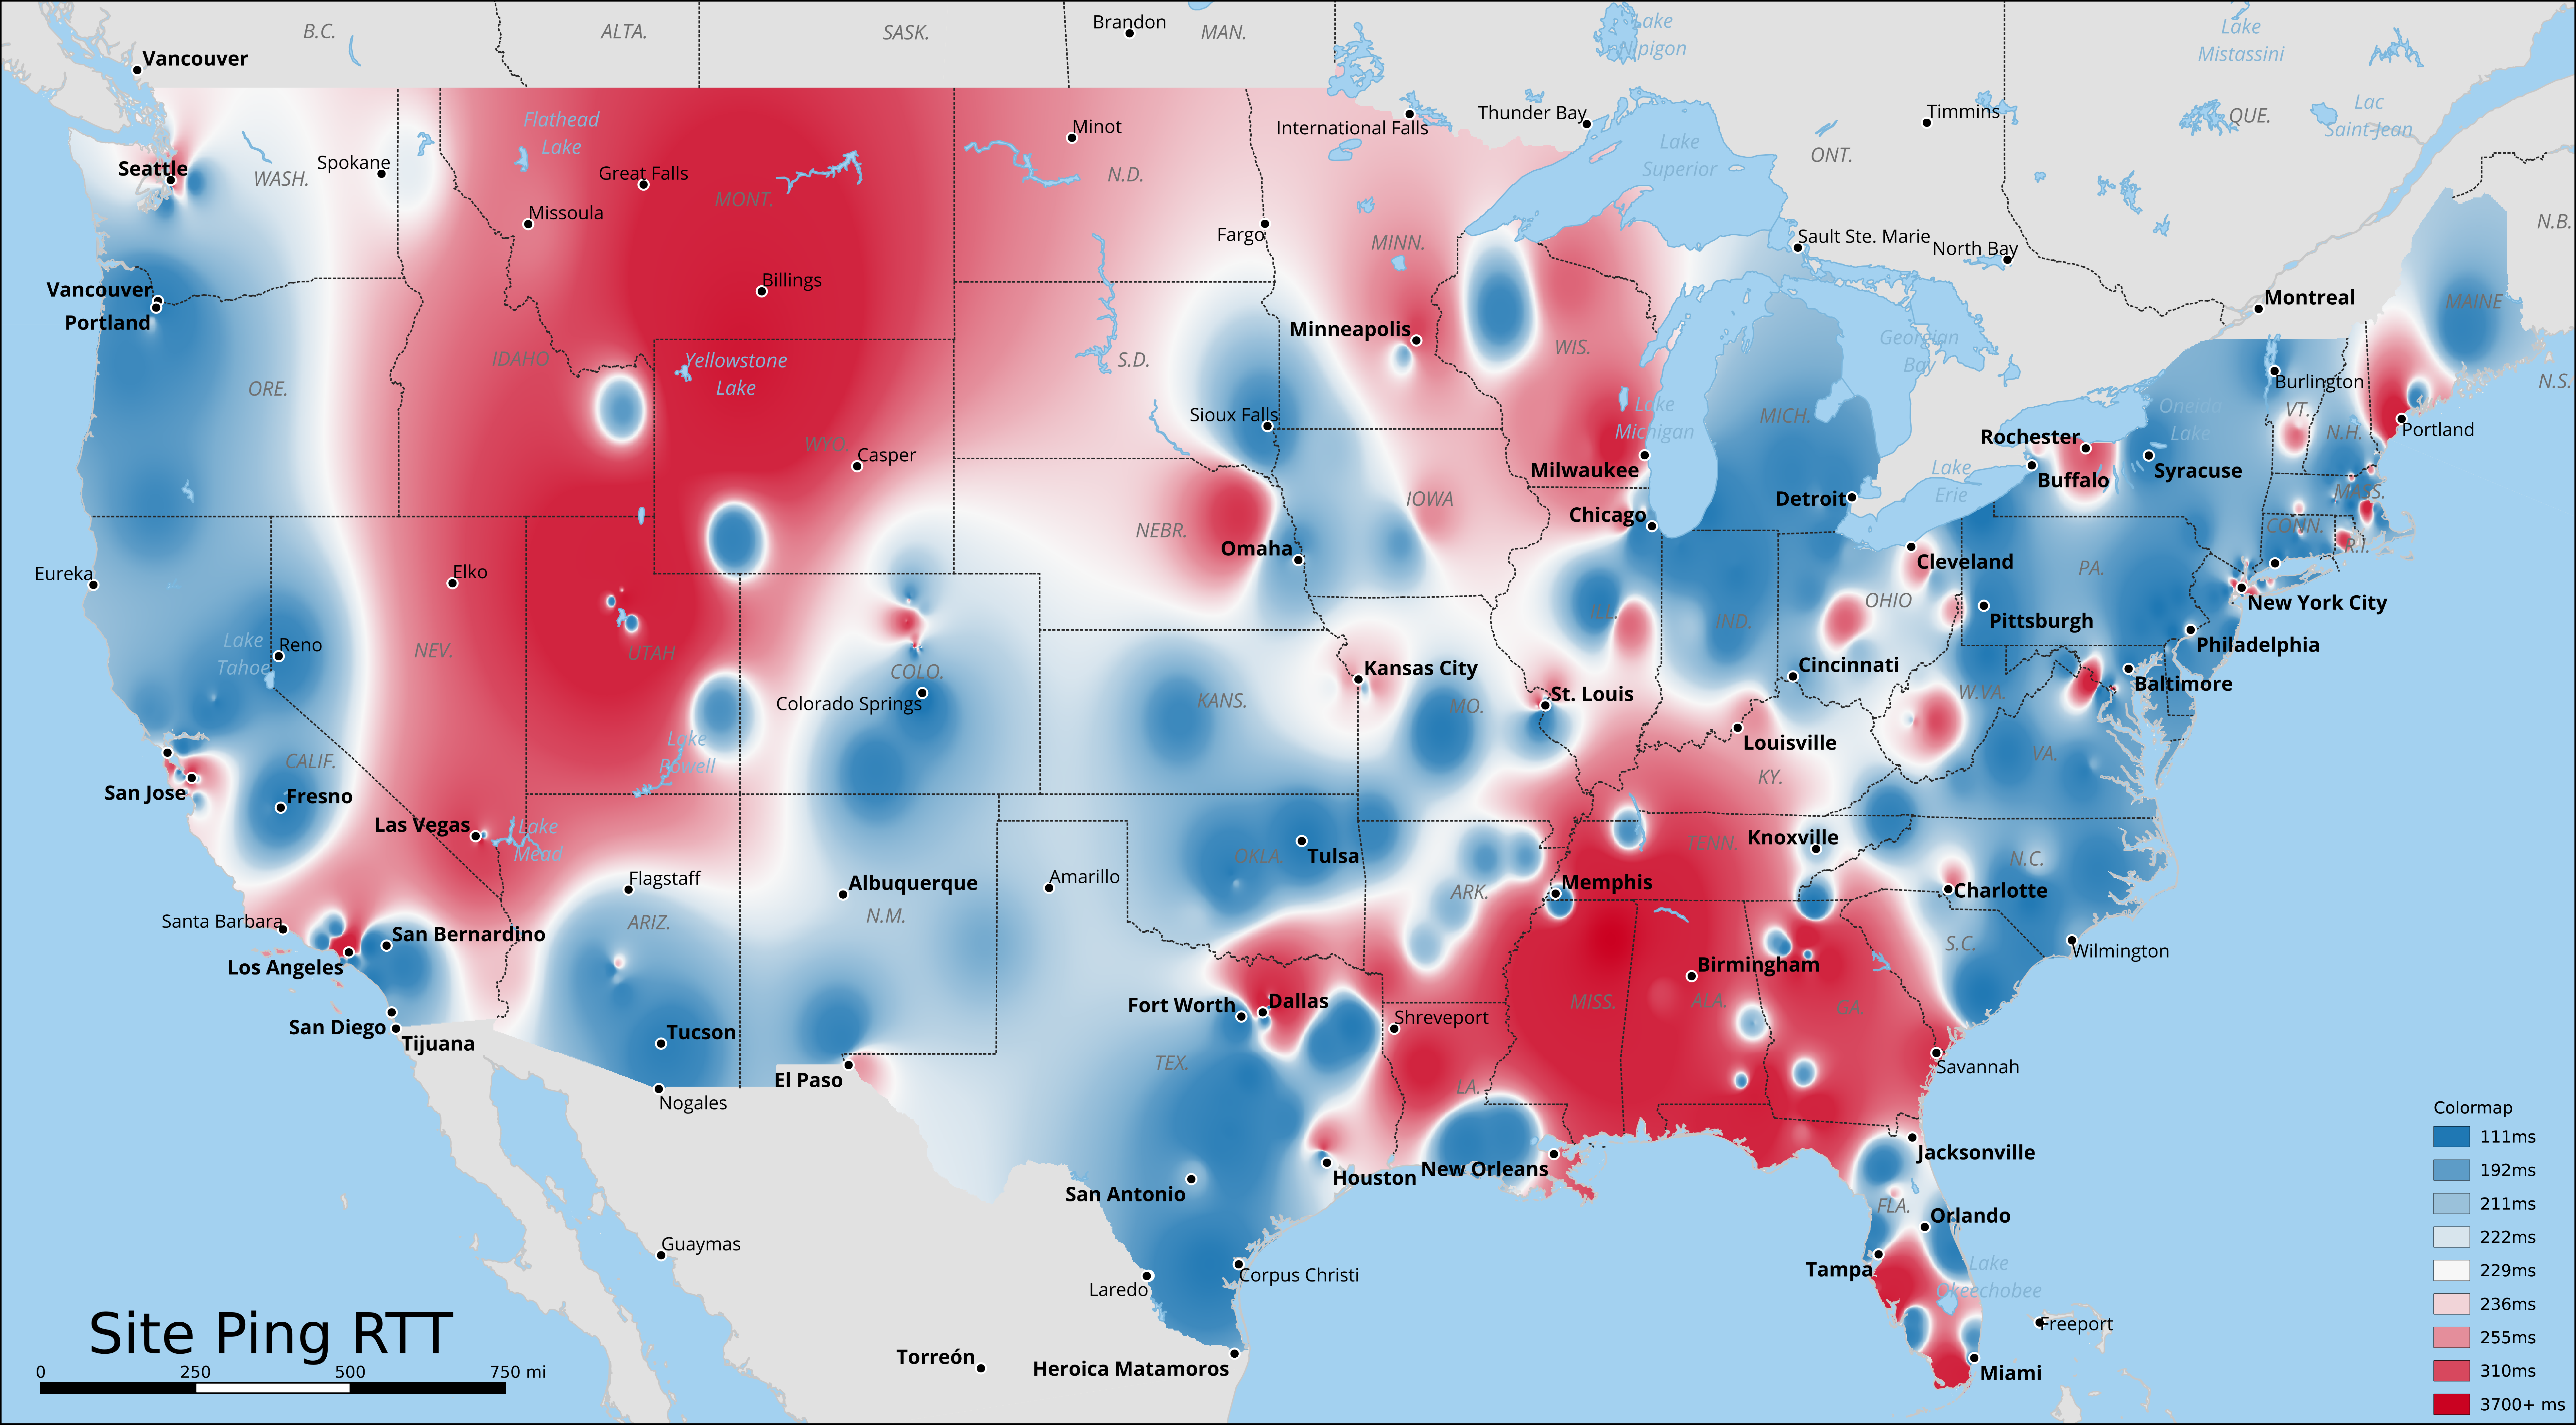
\includegraphics[width=0.85\textwidth]{images/siteping/site_ping_rtt_idw.png}
    \caption{Final Heat Map}
    \label{fig:siteping)_heatmap}
\end{figure}
